\section{Technical Approach}
To infer information about Java code we use existing Java inference tools and 
combine their output. Additionally we have our own framework which allows us to
implement our own analysis. 

To combine all analysis tools (including our own ones) we have to bring 
their results into a common format at some point in our toolchain. 
We will use the JAIF (Java Annotation Index File) format as our common format. 
Firstly because the Javarifier tool generates its output in this file format. 
Secondly because there do exist tools which allow to extract annotations from 
annoted byte code. This makes it easy to use existing tools which embed their 
results into the byte code.

\begin{figure}
\centering
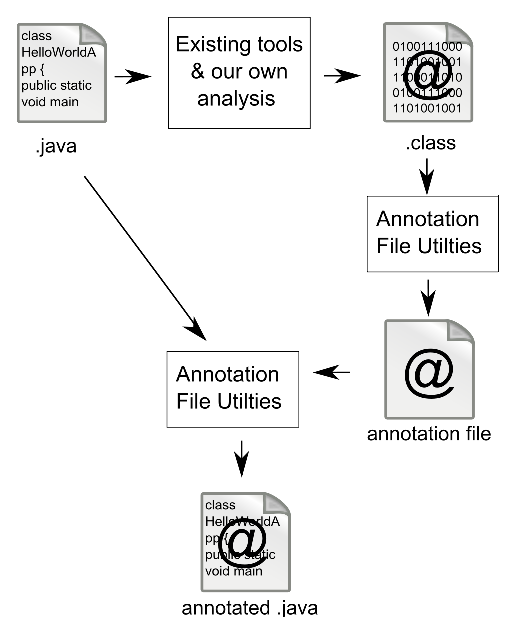
\psfig{file=figures/technicalApproach/technicalApproach.eps, width=3in}
\caption{Toolchain}
\label{fig:toolchain}
\end{figure}

\subsection{Analysis Framework}
\label{ss:analysisFramework}

To implement our own analysis tools we use the current version of the Java 7 compiler.
This allows us to use it's plugin architecture to write our own analyzers. From within
a Java compiler plugin we can access the compiler's abstract syntax tree and we can emit 
annotation to the class files. As described above those annotation will get extracted 
with the annotation file utilities.

In the sections~\ref{sec:Javarifier} until~\ref{sec:Nullability} we show how each analysis 
generates information and transforms it's result to the JAIF format. In the section~\ref{sec:jaif2html}
we explain how we will use all the annotated files to generate a documentation summarizing
the findings of all the analysis techniques.

\subsection{Javarifier}
\label{sec:Javarifier}
TODO Michael


\subsection{Uno}

Uno is an open source tool which is the outcome of a research work done by
Ma and Foster~\cite{Uno}. It infers alias and encapsulation properties for Java.
The tool generates annotations which provide information about how a certain function
treats it's parameters, return objects and fields (in case of a non-static function) 
when called. E.g. if a function captures or leaks a reference or returns a new 
unique reference.

The tool generates annotations which are stored in a single seperate file. We plan
to either change the output mechanism of the tool in a way that it directly generates
JAI files or to write a rewriter which transforms files from Uno's file format to the
JAIF format.

In case we realise that the tool is not fulfilling our needs we will implement
our own (simpler) analysis based on the uniqueness inference algorithm
described in~\cite{UniquenessInference}.

\subsection{Precondition/Dependency}

TODO Colin

\subsection{Nullability}
\label{sec:Nullability}
TODO Gilbert


\subsection{From JAIF to HTML documentation}
\label{sec:jaif2html}

To get the inferred information back into the source files we use the annotation 
file utilities (\cite{AFU} AFU). The next step is to run JavaDoc over our
annotated source code. We will need to write a JavaDoc plugin (called doclet) which will
cause JavaDoc to generate documentation for our new annotations. The output will
generate a HTML documentation of the code enriched with automatically inferred
properties expressed in a programmer friendly format.

Figure \ref{fig:toolchain} shows the stages in our toolchain.